\documentclass[11pt]{article}
\usepackage[T1]{fontenc}
\usepackage{lmodern}
\usepackage[letterpaper,margin=0.9in]{geometry}
\usepackage{graphicx}
\usepackage[hidelinks]{hyperref}
\usepackage{microtype}
\hypersetup{pdftitle={When recovering more tracks creates false counts},pdfauthor={Rushikesh Hulage}}
\title{When recovering more tracks creates false counts\\[4pt]
\large A controlled study of track initiation and line-crossing counts}
\author{Rushikesh Hulage\\[2pt]\normalsize Independent researcher}
\date{November 2026}

\begin{document}
\maketitle
\begin{abstract}
Lowering an online tracker's initiation threshold can recover a valid line crossing and can also turn persistent false detections into a count. We compare initiation thresholds of 0.60 and 0.55 in VisionTrack while holding detections, confirmation and the counting rule fixed within each pair. Across 54 scripted cases, the lower threshold recovers at least one true crossing in 10 cases and violates a prespecified regression criterion in six. In a matched pair of scenarios, identical detections produce identical tracker observations and a crossing that is scored as correct with a reference object and false with an empty reference. A separate scenario preserves a track ID across a detection gap and still misses the crossing. The saved per-frame records support retaining the baseline under the stated decision rule. The prevalence of these failures on traffic cameras remains unmeasured.
\end{abstract}

\section{Introduction}
Line counters use a sequence of public track observations to emit events. Starting a track earlier can provide enough observations to count an object before it passes the line. Persistent false detections can supply the same observations. A track can also survive internally through a detection gap while providing no public observations during that gap, leaving the counter without the adjacent frames it requires.

We use a paired study to trace each outcome from a change in the initiation threshold to an emitted or missed count. The contribution is a reproducible configuration decision for a specified tracker and counting rule, including an identical-input pair that exposes the limits of deciding from those detections alone.

\section{Related work}
ByteTrack associates lower-scoring detections with existing tracks and initiates tracks from unmatched high-scoring detections \cite{bytetrack}. TrackTrack suppresses spurious initiation candidates using overlap with active tracks and stronger detections \cite{tracktrack}. Our experiment changes the birth threshold for proposals that already qualify for VisionTrack's high-score association stage.

HOTA measures detection, association and localization quality \cite{hota}. The AI City vehicle-counting protocol scores cumulative counts by vehicle class and movement over time \cite{aicity}. Liu et al.\ link missed detections and ID switches to counting errors in a movement-specific system \cite{liu}. The TrafficLens artifact already compares counting errors on a fixed real detection stream and isolates an association-threshold change \cite{trafficlens}. Our controlled comparison concerns track birth and uses the same observations with two reference outcomes to trace a specific decision. Each artifact uses its own event rules and data.

\newpage
\section{Method}
We compare VisionTrack's \texttt{new\_track\_thresh} at 0.60 and 0.55. The high-score association threshold is 0.50, confirmation requires three matched observations, and the maximum track age is 30 frames. All other settings are held fixed. The candidate threshold was motivated by an exploratory rain replay. The scripted protocol was fixed before executing this study.

The 54 pairs span nine scripted scenarios, proposal scores of 0.54, 0.57 and 0.61, and speeds of 2 and 6 pixels per frame. The tracker receives class, score and bounding box. Reference boxes are used separately during scoring. The counter emits an event when centers of two boxes for the same public ID in adjacent frames cross \(x=500\) from left to right within \(205 \le y \le 432\). We match predictions one to one with references within one frame and 10 pixels of crossing height. Matching maximizes cardinality and then minimizes time error.

A change qualifies for further consideration if it recovers a true crossing and leaves all four regression measures at or below baseline in every case. The measures are false public boxes, false crossing events, ID switches and extra matched IDs. For each reference object, the last measure counts distinct matched IDs beyond the first. Public boxes are scored at an intersection-over-union threshold of 0.5. We use three passes per variant (fresh, reset, fresh) to check repeatability, for 324 tracker passes in total.

\begin{figure}[h!]
\centering
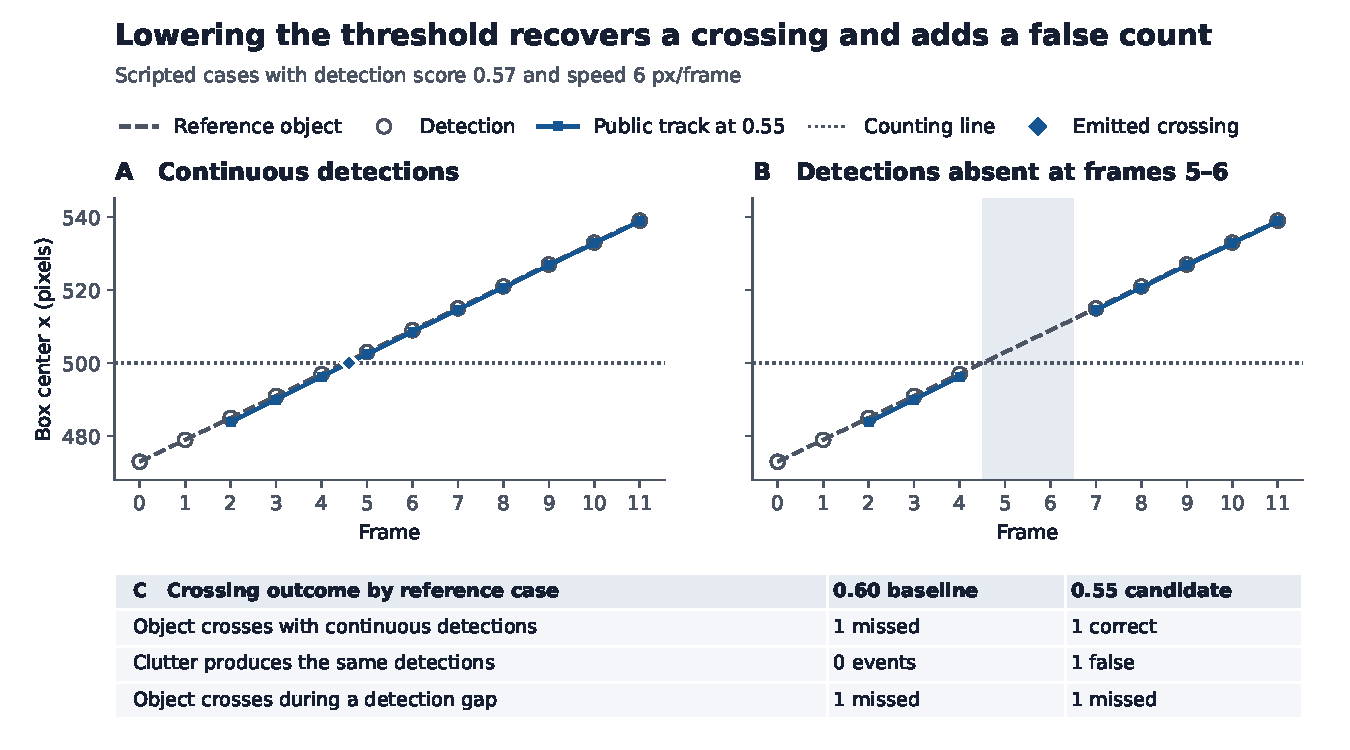
\includegraphics[width=\linewidth]{initiation-threshold.pdf}
\caption{\textbf{A.} With continuous detections, the lower threshold confirms the track at frame 2 and counts a crossing between frames 4 and 5. The clutter case produces the same observations with an empty reference. \textbf{B.} The candidate reports the same ID before and after a gap at frames 5 and 6, leaving no adjacent pair spanning the line. \textbf{C.} The event is correct with the reference object and false with the empty reference. Both thresholds miss the gap crossing. These outcomes also hold at 2 pixels per frame.}
\label{fig:crossings}
\end{figure}

\newpage
\section{Results and limitations}
The 0.55 setting recovers at least one true crossing in 10 paired cases and violates at least one regression criterion in six. Across the scripted cases, correct counts rise from 18 to 30, missed crossings fall from 30 to 18, and false counts rise from 4 to 8. Four of the six regressions are persistent-clutter cases and two involve an absence longer than the track lifetime. All 36 controls at scores 0.54 and 0.61 have identical tracker outputs under both configurations.

Figure~\ref{fig:crossings} isolates two ways the same threshold decision can affect a counter. In the continuous object and clutter cases, both the detection streams and the tracker outputs are identical across the two scenes for each threshold. The reference determines whether the event is a correct count. In the detection-gap case, the preserved ID still leaves a discontinuity in public observations, so the counter misses the reference crossing.

We retain the 0.60 setting under the stated criterion. These authored scenarios describe mechanisms in one tracker and one counter. They give no estimate of their frequency in traffic, and a detector or a counter with different temporal rules could change the outcome. A field assessment would require separately evaluated cameras and independently checked crossing labels.

\section{Reproducibility}
The \href{https://github.com/hulagerushikesh/visiontrack/blob/b4ccff0dc415e9755c1dc2448d3b3defc5a87481/docs/INITIATION_THRESHOLD_FINDINGS.md\#reproduce-the-study-and-figure}{pinned replay instructions} verify all 54 pairs against the \href{https://github.com/hulagerushikesh/visiontrack/blob/898593aed4111fff38c872807d7299581d6f8de2/experiments/initiation_threshold_v1_results.json}{scored summary} and regenerate Figure~\ref{fig:crossings}. The \href{https://github.com/hulagerushikesh/visiontrack/blob/4b44af0abb0c7448f6baf796e5cfa1062d52f6a6/docs/INITIATION_THRESHOLD_PROTOCOL.md}{frozen protocol and executable snapshot} generate the inputs without footage or model weights. With Python 3.12.9, NumPy 2.5.4 and Matplotlib 3.10.9, macOS ARM64 and two Linux containers (ARM64 and emulated x86-64 on the same Apple Silicon host) reproduced all 216 per-case files and the figure SVG byte for byte. The \href{https://visiontrack.hulage.in/lab/crossings\#controlled-threshold}{Reliability Lab} shows selected results.

\paragraph{Use of AI tools.} OpenAI Codex and Anthropic Claude assisted with implementing and replaying the experiments, verifying outputs, generating the figure, and drafting, editing and typesetting the manuscript. The author reviewed all content and is responsible for it.

\paragraph{License.} This manuscript is distributed under the Creative Commons Attribution 4.0 International license (\href{https://creativecommons.org/licenses/by/4.0/}{CC BY 4.0}). The VisionTrack code is released under the MIT license.

\begin{thebibliography}{9}
\small
\bibitem{bytetrack}
Y. Zhang et al. \href{https://arxiv.org/abs/2110.06864}{ByteTrack: Multi-Object Tracking by Associating Every Detection Box}. ECCV, 2022.
\bibitem{tracktrack}
K. Shim, K. Ko, Y. Yang, and C. Kim. \href{https://openaccess.thecvf.com/content/CVPR2025/html/Shim_Focusing_on_Tracks_for_Online_Multi-Object_Tracking_CVPR_2025_paper.html}{Focusing on Tracks for Online Multi-Object Tracking}. CVPR, 2025.
\bibitem{hota}
J. Luiten et al. \href{https://pmc.ncbi.nlm.nih.gov/articles/PMC7881978/}{HOTA: A Higher Order Metric for Evaluating Multi-Object Tracking}. International Journal of Computer Vision, 2021.
\bibitem{aicity}
AI City Challenge. \href{https://www.aicitychallenge.org/2021-data-and-evaluation/}{2021 Data and Evaluation, Track 1}.
\bibitem{liu}
Z. Liu et al. \href{https://openaccess.thecvf.com/content_CVPRW_2020/papers/w35/Liu_Robust_Movement-Specific_Vehicle_Counting_at_Crowded_Intersections_CVPRW_2020_paper.pdf}{Robust Movement-Specific Vehicle Counting at Crowded Intersections}. CVPR Workshops, 2020.
\bibitem{trafficlens}
TrafficLens. \href{https://github.com/safdar-hussain1/trafficlens/blob/9aef029c68a9c7dc4c0f112085418483ddbb985c/README.md\#measured-results}{Measured Results and Ablations}. Project documentation, revision \texttt{9aef029}.
\end{thebibliography}
\end{document}
